\documentclass[conference]{IEEEtran}

\usepackage{hyperref}
\usepackage{graphicx}
\usepackage{fancyhdr}
%\usepackage{lastpage}
\usepackage{amsmath}
\usepackage{amscd}
\usepackage{color}
\usepackage{url}
%\usepackage{moreverb}
\usepackage{verbatim}
\usepackage{textcomp}
\usepackage{mathptmx}
\usepackage{dingbat}
\usepackage{pifont}
\usepackage{acronym}
\usepackage{algpseudocode}
\usepackage{algorithm}
\usepackage{supertabular}
\usepackage{listings}
\usepackage{threeparttable}
\usepackage{pdflscape}
\usepackage{array}
\usepackage{multirow}
\usepackage{subfigure}

\usepackage[numbers,sort]{natbib}

\renewcommand{\algorithmiccomment}[1]{\hfill {\tt //} #1}
\newcommand{\tick}{\ding{52}}
\newcommand{\xmark}{\ding{56}}

\date{}
\begin{document}

\author{
\IEEEauthorblockN{Dimitris Mitropoulos,\IEEEauthorrefmark{1}
Panos Louridas,\IEEEauthorrefmark{2} and Angelos Keromytis\IEEEauthorrefmark{1}}
\IEEEauthorblockA{\IEEEauthorrefmark{1}
Network Security Lab\\
Department of Computer Scinence\\
Columbia University\\
\{dimitro, angelos\}@cs.columbia.edu\\
\IEEEauthorrefmark{2}
Software Engineering and Security Lab\\
Department of Management Science and Technology\\
Athens University of Economics and Business\\
louridas@aueb.gr
}}

\title{SoK: Web Application Attack Defenses (in Question)}

\maketitle
\begin{abstract}
In this paper we examine how application attack defense
mechanism are developed and presented to
the research community.
\end{abstract}

\begin{IEEEkeywords}
Security and Protection, Application Security, Code injection Attacks, Cyber Security Experiments, Effectivenes, Efficiency.
\end{IEEEkeywords}

\IEEEpeerreviewmaketitle

\section{Introduction}

Introduction~\cite{I05}. Also see~\cite{A00}.

Requirements:
\begin{itemize}
\item {\bf Flexibility} We check if an approach
can be adjusted in order to detect different {\sc cia} categories.
\item {\bf Ease of use} We examine if the mechanism that
implements an approach is practical and can be easily adopted
by security experts.
\item {\bf Effectiveness} As long as we examine security
mechanisms that detect either attacks or defects,
the non-existence of false positive and negative alarms
is a reasonable requirement.
\item {\bf Efficiency} Finally, we examine
the computational overhead of the mechanisms that affect the experience of
a web user who actually uses the protected application.
\item {\bf Security} How resilient is the system to
attacks made to to circumvent it.
\end{itemize}
All the aforementioned requirements are considered critical
when building security mechanisms that protect
applications~\cite{A01,A00}.

\section{Attacks}
\label{sec:attacks}

The basic problem behind web application attacks involves
the absence of input validation. By taking advantage of
this, attackers can inject either code into
applications to perform malicious tasks. Such
an exploit can have different forms depending on the
execution context of the application and the location
of the programming flaw that leads to the attack.

Bratus et al.~\cite{BLSPS11} portray the issue in a generic fashion:
{\it ``unexpected (and unexpectedly powerful) computational models
inside targeted systems, which turn a part of the target into a
so-called ``weird machine" programmable by the attacker via crafted inputs
(a.k.a. ``exploits")"}.
An example of the above definition is the
following: The code fragment below, defines the operation of
addition in the Scheme programming language~\cite{AS96,D09}:

\begin{verbatim}
(define (add x y) (+ x y))
\end{verbatim}

\noindent
Consider the case where instead of a number, a function that leads to an
endless loop is passed as an argument by the user. This will cause
the interpreter to enter
an endless loop and lead to a denial of service.
% Keep in mind that a {\sc cia} does not require a programming
% language with first-class functions.
The intuition here is that {\it ``every application that copies
untrusted input verbatim into an output
program is vulnerable to code injection"}.
Ray and Ligatti~\cite{RL12b} actually proved the above
claim based on formal language theory.

\begin{figure}
\begin{center}
\leavevmode
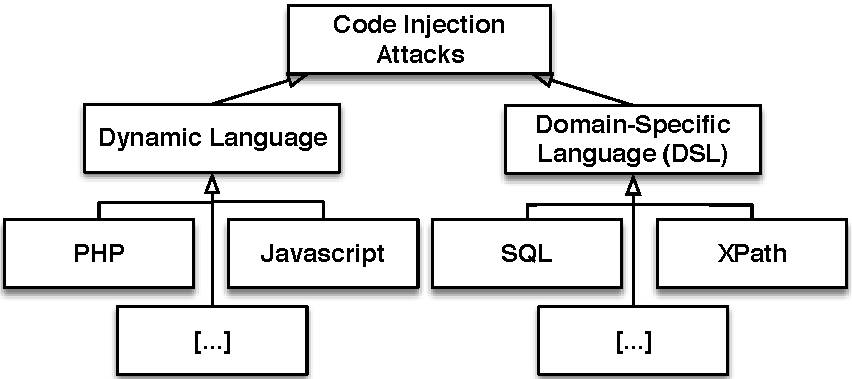
\includegraphics[scale=0.37]{attack-tree-uml.pdf}
\end{center}
\caption{\label{fig:taxonomy}A taxonomy of code injection attacks.
In our research we have excluded the defenses that deal with
the subcategories that are illustrated in grey color.}
\end{figure}

Figure \ref{fig:taxonomy} presents a taxonomy of code injection attacks divided
into two categories. The first involves binary code and the second
executable source code.

\subsection{Binary Code Injection}

Binary code injection attacks involve
the insertion of binary code into an application
to alter its execution flow and execute malicious
compiled code. This category involves buffer-overflow
attacks~\cite{CPMHWBBGWZ98,K11}, a staple of security problems.
An extensive survey on binary code
injection attacks can be found in reference~\cite{LC03}.
Furthermore, specific advances in exploiting such vulnerabilities
(i.e. ``heap smashing", ``arc injection" and others)
have been presented in reference~\cite{PB04}.
Finally, the countermeasures used to detect
such defects have already been surveyed~\cite{YJP12}
(many of them are also included in a book:~\cite{DKZ12}
-- Section 13.8), thus we do not include them in our work.

\subsection{Executable Source Code Injection}

Code injection also includes the use of source code, either of a
Domain Specific Language ({\sc dsl})
or a Dynamic Language. Note that binary code injection
attacks can only occur when the target system is implemented in
languages lacking array bounds checking, like
{\sc c} and {\sc c}++. Contrariwise, source code-driven
injection attacks can target applications written in various
programming languages with different features and characteristics.

Application attacks that involve {\sc dsl}s,
constitute an important subset of the code injection problem,
as {\sc dsl}s like {\sc sql} and {\sc xml} play an
significant role in the development of either web or mobile
applications. For example, many applications have interfaces
where a user enters input to interact with the
application's data, thereby interacting with the
underlying {\it Relational Database Management System}
({\sc rdbms}).
This input can become part of an
{\sc sql} query and executed on the target {\sc rdbms}.
A code injection attack that exploits the vulnerabilities of these
interfaces by taking advantage of input validation issues like
incorrectly passed parameters or incorrect type handling,
is called an ``{\sc sql} injection
attack''~\cite{CERT02,MS09,HVO06,SW06}.
By using similar techniques malicious users
can perform other exploits based on {\sc dsl}s,
like {\sc xp}ath~\cite{SW06,CDL07,MKS09} and
{\sc xml}~\cite{MSM13} injection attacks.

A recent class of {\sc cia}s involve
dynamic languages like Python, Perl, JavaScript, and {\sc php}~\cite{SFVM09,EWKK09,SMS13}.
In particular, JavaScript injection attacks comprise a wide subset of dynamic
language-driven attacks. Such attacks are manifested when a web application
accepts and redisplays data of uncertain origin without appropriate validation
and filtering. Based on this flaw, an attacker can
manage to inject a script in the JavaScript engine of a browser and alter its
execution flow~\cite{ELX07}. JavaScript injection attacks are considered as a
critical issue in web application security mainly because they are
associated with major vulnerabilities such as:
{\sc xss} attacks~\cite{SG07},
{\sc csrf} attacks~\cite{LZRL09}
and ``Cross-Channel Scripting"
({\sc xcs}) attacks~\cite{W10,BBB09}.

\section{Defenses for Detecting Web Application Attacks}

There are four main defensive approaches to counter
web application attacks, namely: {\it tainting},
{\it instruction set randomization} ({{\sc isr}}),
{\it policy enforcement} and {\it training}. 

\section{Methodological Background}

As in medical diagnostic tests, application attack defense mechanisms
must demonstrate the presence of an attack. This, however, does not
make an application attack defense mechanism immediately useful. In
order for a detection mechanism to be useful it must be accurate, easy to
use, and economical. The accuracy of a detection mechanism is gauged
with the following metrics~\cite{TDR2013,GFDLS06,A00}:
\begin{itemize}
\item {\bf Sensitivity}, the probability that an attack will be
  caught.
\item {\bf Specificity}, the probability that a normal interaction
  will test negative.
\item {\bf Positive Predictive Value} ({\sc ppv}), the probability that a
  reported attack is a real attack. It is the conditional probability
  that an event is an attack if the detection mechanism flags it as
  such. 
\item {\bf Negative Predictive Value} ({\sc npv}), the probability that if
  nothing is reported no attack has taken place. It is the conditional
  probability that an event is not an attack given that the detection
  mechanism flags it as normal.
\end{itemize}

Sensitivity and specifity are defined by way of the $2\times 2$
Table~\ref{tab:sensitivity-specificity}~\cite{linn2004}. 
In the cells of
the table we distinguish:
\begin{itemize}
\item True Positive ($a$), a real attack that raises an alarm.
\item True Negative ($d$), an event that is not an attack and that does
  not raise an alarm.
\item False Positive ($b$), an event that although it is not an attack
  raises an alarm.
\item False Negative ($c$), an event that although is as attack does
  not raise an alarm.
\end{itemize}

\noindent
With these we can calculate:

\begin{equation}
\textrm{SE} = \textrm{Sensitivity} = \frac{a}{a + c}
\end{equation}

\begin{equation}
\textrm{SP} = \textrm{Specificity} = \frac{d}{b + d}
\end{equation}

Sensitivity and specificity can be calculated based on test
data alone. To calculate the sensitivity, we run the test on a
controlled environment where we allow only attack events to reach the
system. The ratio of reported attacks over all attacks will give us
the sensitivity. Similarly, to calculate the specificity we can run
the test on a controlled environment where we allow only innocuous
events to reach the system. The ratio of non-reported events over all
events will give us the specificity. 

\begin{table}[ht]

\caption{Attacks and Test Outcomes in Test Environment}
\label{tab:sensitivity-specificity}

\begin{tabular}{l|l|c|c|}
\multicolumn{2}{c}{} & \multicolumn{2}{c}{Attack} \\ \cline{3-4}
\multicolumn{2}{c|}{} & Yes & No \\ \cline{2-4}
\multirow{2}{*}{Result} &  Yes &  $a = \textrm{True Positive}$ & 
$b = \textrm{False Positive}$ \\
& No & $c = \textrm{False Negative}$ & $d = \textrm{True Negative}$ \\ 
\cline{2-4}
\multicolumn{2}{r|}{Total} & $a + c$ & $b + d$ \\
\cline{3-4}
\end{tabular}

\end{table}

Note that the calculations are carried out vertically in
Table~\ref{tab:sensitivity-specificity}; the ratio of attack events to
normal events does not enter into sensitivity and specificity. This is
what allows us to derive them based on test data, without using data
from a real production environment. At the same time, however, this is
what limits their usefulness. When we obtain a test result in a
production environment, be it negative or positive, we really want to
know how much we should be worried, or relaxed. In other words, if an
attack is detected in a production environment, how much should we be
worried? If no attack is detected in a production environment, how
relaxed should we be that no attack has indeed taken place?

\begin{table}[ht]

\caption{Attacks and Test Outcomes in Real Environment}
\label{tab:ppv-npv}

\begin{tabular}{l|l|c|c|c}
\multicolumn{2}{c}{} & \multicolumn{2}{c}{Attack} & \\ \cline{3-4}
\multicolumn{2}{c|}{} & Yes & No & Total \\ \cline{2-5}
\multirow{2}{*}{Result} &  Yes &  $A = \textrm{True Positive}$ & 
$B = \textrm{False Positive}$ & \multicolumn{1}{c|}{$A + B$}\\
& No & $C = \textrm{False Negative}$ & $D = \textrm{True Negative}$ &
\multicolumn{1}{c|}{$C + D$}\\ 
\cline{2-5}
\end{tabular}

\end{table}

The answer to these questions is given by the \textsc{ppv} and the
\textsc{npv}. These depend not only on the test results, but also on
the \emph{prevalence} of attacks in real environments. In particular,
we can calculate them using Table~\ref{tab:ppv-npv}, which tabulates
results in a real environment, or in an environment where the
prevalence of attacks is equal to what we expect in the real world. To
indicate the difference with Table~\ref{tab:sensitivity-specificity}
we use capital letters for the entries in the table~\cite{linn2004}.
With this table, \textsc{ppv} and \textsc{npv} are given by the
following equations:

\begin{equation}
\textrm{PPV} = \frac{A}{A + C}
\end{equation}

\begin{equation}
\textrm{NPV} = \frac{D}{B + D}
\end{equation}

This time the ratios are taken horizontally; the ratio of attacks to
innocuous events affects the calculations. In fact, if PR is the
probability of attacks in the real world, the prevalence, then we
have~\cite{linn2004,altman1994}:

\begin{equation}
\textrm{PPV} = \frac{\textrm{SE}\times \textrm{PR}}{
\textrm{SE}\times \textrm{PR} + (1 - \textrm{SP})\times (1 -
\textrm{PR})}
\label{eq:ppv-se-sp}
\end{equation}

\begin{equation}
\textrm{NPV} = \frac{\textrm{SP}\times (1 - \textrm{PR})}{
(1 - \textrm{SE})\times \textrm{PR} + \textrm{SP}\times (1 -
\textrm{PR})}
\label{eq:npv-se-sp}
\end{equation}

The prevalence is the prior probability that an event is an attack,
based on our understanding of the volume and frequency of attacks; the
\textsc{ppv} and \textsc{npv} are the revised estimates of the
probability based on the results of the detection
mechanism~\cite{altman1994}. The lower the prevalence of an attack,
the more confident we can be that a negative test result indicates
that no attack has taken place and the less sure we can be that a
positive test result indicates a real attack. 

In what follows we evaluate published research in attack detection
mechanism based on the following:
\begin{itemize}
\item \textbf{Sensitivity, Specificity}: Reporting of values for True
  Positives ($a$), False Positives ($b$), False Negatives ($c$), True
  Negatives ($d$), on test environments.
\item \textbf{\textsc{ppv}, \textsc{npv}}: Reporting of values for True
  Positives ($A$), False Positives ($B$), False Negatives ($C$), True
  Negatives ($D$), on the performance of the mechanism on environments
  with real attack profiles. Alternatively, since from
  equations~\ref{eq:ppv-se-sp} and~\ref{eq:npv-se-sp} \textsc{ppv}
  and \textsc{npv} can be calculated by the sensitity and specifity
  given the prevalence, reporting of prevalance, sensitivity,
  specificity.
\end{itemize}

\section{Covered Area}

We decided to narrow down our
research to countermeasures developed to
detect attacks that target applications. Such attacks include
buffer overflow attacks~\cite{K11}, {\sc sql} injection
attacks~\cite{RL12b}, cross-site scripting ({\sc xss})
attacks~\cite{SG07}, cross-site request forgery ({\sc csrf})
attacks~\cite{LZRL09} and others.
Such attacks top the vulnerability lists of numerous bulletin providers for several
years.\footnote{\url{http://www.sans.org/top-cyber-security-risks/}, \url{http://cwe.mitre.org/top25/}}
Consider the {\sc owasp}\footnote{\url{https://www.owasp.org/index.php/Category:OWASP_Top_Ten_Project}}
(Open Web Application Security Project)
Top Ten project whose main goal is to raise awareness about
web application security by identifying some of the most critical risks facing
organizations which is referenced by numerous researchers.
In its three consecutive Top Ten lists (2007, 2010, 2013), different
source code-driven injection attacks dominate the top five positions.
This indicates that
apart from the fact that malicious users find new ways to bypass
defense mechanisms by using a variety of techniques despite the numerous
countermeasures that are being introduced.
Note that the number of systems developed to counter {\sc sql}
injection attacks until 2006 was more than twenty~\cite{HVO06}.
Since then the number has doubled.
In our research we focus on the top {\sc tba} systems that counter
application attacks, in terms of citations.
% TODO@dimitro: explain why you leave out {\it SecuriFly}~\cite{MLL05}.

\begin{landscape}
\begin{table}
%\tbl{Performance of System Prototype. Time is Measured in $\mu$s.}{
\centering
    \begin{threeparttable}
    \begin{small}
\scalebox{0.99}{
    \begin{tabular}{l|c|c|cc|c}
    \hline
    \bf{Approach}
	& \bf{Mechanism}
	& \bf{\# of Citations}
    & \multicolumn{2}{|c|}{Requirements\tnote{1}}
	& \bf{Attack} \\
	&&& \bf{TP,TN,FP,FN}\tnote{2}
	& \bf{Computational Overhead} & \\
    \hline
	\multirow{9}{*}{Runtime Tainting}
  &   {\it Haldar et al.}~\cite{HCF05} & 177 & (2,{\sc na},{\sc na},0)\_s & {\sc nq} & {\sc sql} injection, {\sc xss} \\ 
	&  	{\sc csse}~\cite{PB05} & 312 & (7,{\sc nq},{\sc nq},{\sc nq})\_r & 2--10\% & {\sc sql} injection, {\sc xp}ath, {\sc xss} \\
	% &  	{\it SecuriFly}~\cite{MLL05} & 31 & \xmark,\tick & 9--125\% & {\sc sql} injection, {\sc xss} \\ 
	&  	{\it Xu et al.}~\cite{XBS06} & 297 & (9,{\sc nq},0,{\sc nq})\_r & average 76\% & {\sc sql} injection, {\sc xss} \\ 
    &  	{\it {\sc wasc}}~\cite{NLC07} & 31 & ({\sc nq},{\sc nq},{\sc nq},{\sc nq})\_r & up to 30\% & {\sc sql} injection, {\sc xss} \\
	&  	{\it Vogt et al.}~\cite{VFJKKV07} & 322 & ({\sc nq},{\sc nq},{\sc nq},{\sc na})\_r & {\sc nq} & {\sc xss} \\
	&   {\it Noxes}~\cite{KKVJ06,KJKV09} & 268,40 & (3,{\sc na},{\sc na},0)\_r & {\sc na} & {\sc xss} \\
	&  	{\it {\sc php} Aspis}~\cite{PMP11} & 12 & (15,{\sc nq},{\sc nq},{\sc nq})\_r & 2.2$\times$ & {\sc sql} and {\sc php} injection, {\sc xss} \\
	& 	{\it Stock et al.}~\cite{SLMS14} & 0 & (1169,{\sc na},{\sc na},0)\_r & 7--17\% & {\sc dom}-based {\sc xss} \\
	\hline
	\hline      
	\multirow{3}{*}{{\sc isr}}
	&   {\it {\sc sql}rand}~\cite{BK04} & 286 & (3,{\sc na},{\sc na},0)\_a & +6.5{\it ms} & {\sc sql} injection \\ 
	&   {\it Noncespaces}~\cite{GC09} & 109 & ({\sc nq},{\sc na},{\sc na},0)\_r &  10.3\% & {\sc xss} \\ 
    &   {\it x{\sc js}}~\cite{APKLM10} & 18 & (1380,{\sc na},{\sc na},1)\_r & 1.6--40{\it ms} & {\sc xss} \\
	\hline
	\hline    
	\multirow{12}{*}{Policy Enforcement}
	&   {\it {\sc dsi}}~\cite{NSS06} & 135 & (5268,{\sc nq},46,15)\_r & 1.85\% & {\sc xss} \\ 
	&   {\it BrowserShield}~\cite{RDWDE07} & 219 & (19,{\sc nq},0,0,)\_r & 8\% & {\sc xss} \\ 
	&   {\it CoreScript}~\cite{YCIS07} & 181 & ({\sc nq},{\sc nq},{\sc nq},{\sc na})\_s & {\sc nq} & {\sc xss} \\ 
	&   {\it {\sc met}}~\cite{ELX07} & 58 & ({\sc na},{\sc na},{\sc na},{\sc na})\_{\bf ?} & {\sc na} & {\sc xss} \\ 
    &   {\it {\sc beep}}~\cite{TNH07} & 282 & (61,{\sc na},{\sc na},0)\_r & 14.4\% & {\sc xss} \\
    &   {\it {\sc soma}}~\cite{OWVS08} & 46 & (5,{\sc na},{\sc na},0)\_s & 5.58\% & {\sc xss}, {\sc csrf}\\
	&   {\it Blueprint}~\cite{LV09} & 110 & (94,{\sc na},{\sc na},0)\_r & 13.6\% & {\sc xss} \\ 
	&   {\it Phung et al.}~\cite{PSC09} & 75 & (37,{\sc na},{\sc na},4)\_r & 5.37\% & {\sc xss} \\
	&   {\it WebJail}~\cite{VDDPJ11} & 25 & ({\sc na},{\sc na},{\sc na},{\sc na})\_{\bf ?} & $\sim$7ms & {\sc xss} \\ 
	&   {\it ConScript}~\cite{ML10} & 122 & ({\sc na},{\sc na},{\sc na},{\sc na})\_{\bf ?} & 7\% & {\sc xss} \\
	&   {\it j{\sc csrf}}~\cite{PS11} & 2 & (2,{\sc na},{\sc na},0)\_r & 2ms & {\sc csrf} \\
    &   {\it TreeHouse}~\cite{IW12} & 18 & ({\sc na},{\sc na},{\sc na},{\sc na})\_{\bf ?} & 757–-1218ms & {\sc xss} \\
   	% &   {\it {\sc js}and}~\cite{AVBPDP12} & 22 & ({\sc na},{\sc na},{\sc na},{\sc na})\_{\bf ?} & up to 31.2\% & {\sc xss}\\
   	% TODO@dimitro: discuss this with Panos?
	\hline
	\hline  
        \multirow{11}{*}{Training}
    &   {\it {\sc didafit}}~\cite{LLW02} & 85 & ({\sc na},{\sc na},{\sc na},{\sc na})\_{\bf ?} & {\sc na} & {\sc sql} injection \\
	&   {\it {\sc amnesia}}~\cite{HO05,HO06,HO05b} & 118,66,376 & (1470,{\sc nq},0,0)\_a & {\sc nq} & {\sc sql} injection \\ 
	&   {\it libAnomaly}~\cite{VMV05} & 226 & (344,15646,60,0)\_r & +1{\it ms} & {\sc sql} injection \\
	& 	{\it {\sc sqlg}uard}~\cite{BWS05} & 243 & ({\sc na},{\sc na},{\sc na},{\sc na})\_{\bf ?} & 3\% & {\sc sql} injection \\
	& 	{\it {\sc sm}ask}~\cite{JB07} & 27 & (5,{\sc nq},{\sc nq},{\sc nq})\_r  & {\sc na} & {\sc sql} injection, {\sc xss} \\
	& 	{\it {\sc xssds}}~\cite{JEP08} & 64 & ({\sc nq},{\sc nq},{\sc nq},0)\_r & {\sc nq} &  {\sc xss} \\
    & 	{\it {\sc xss-guard}}~\cite{BV08} & 97 & (8,{\sc nq},{\sc nq},{\sc nq})\_r & 5--24\% & {\sc xss} \\
    & 	{\it {\sc swap}}~\cite{WPLKK09} & 52 & ({\sc nq},{\sc nq},{\sc nq},{\sc nq})\_r & $\sim$180\% & {\sc xss} \\ 
	& 	{\it {\sc sd}river}~\cite{MS09,MKS09,MKLS11} & 20,8,5 & (241,{\sc nq},0,0)\_a & 39\% & {\sc sql} and {\sc xp}ath injection \\
	% & 	{\it Laranjeiro et al.}~\cite{LVM09,ALVM09,LVM10} & 9,40,1 & \xmark,\xmark  & \xmark & {\sc sql} and {\sc xp}ath injection \\
	& 	{\it Diglossia}~\cite{SMS13} & 3 & (9,{\sc nq},{\sc nq},{\sc nq})\_r & 13\% & {\sc sql} and No{\sc sql} injection \\
	\hline
    \end{tabular}}
    \begin{tablenotes}
	\begin{footnotesize}
       	\item[1] {\sc na} (Not Available) means that a requirement is not even mentioned in the paper.
	{\sc nq} (Not Quantified) indicates that a requirement is mentioned in the publication
	but it is not quantified.
		\item[2] For every quadruple there is a corresponding suffix that indicates whether the testbed was
	based on real-world applications known to be vulnerable ({\it r}), synthetic benchmarks ({\it s}) or both ({\it a}).
	If no testing has taken place we add a question mark ({\bf ?}).
	\end{footnotesize}
    \end{tablenotes}
    \caption{Comparison summary of mechanisms developed to counter application attacks.}
    \label{tab:comp2}
    \end{small}
    \end{threeparttable}
\end{table}
\end{landscape}

\section{Analysis}

Notes on taint tools:
\begin{enumerate}
\item The accuracy testing of {\sc csse}~\cite{PB05} was based on 
defects found in the security mailing
list: {\it Bugtraq}\footnote{\url{http://seclists.org/bugtraq/}}.
\item During their evaluation, the authors of~\cite{HCF05} have only performed
two attacks in one synthetic benchmark ({\sc owasp}'s
{\it WebGoat}\footnote{\url{https://www.owasp.org/index.php/Category:OWASP_WebGoat_Project}}).
\item The testing in~\cite{XBS06} was made based on
defects with specific {\sc cve id}s.
\item The authors of {\it {\sc wasc}}~\cite{NLC07}
mention the vulnerabilities (specific {\sc cve id}s)
exploited and the corresponding applications but they do not explicitly
state how many attacks they launched (``{\it [...] launched a variety of
attacks against it}").
\item The authors of~\cite{VFJKKV07} do the same.
However, even if they do not mention specific {\sc cve id}s,
they browsed applications without performing attacks.
\item Even if the authors of {\it Noxes}~\cite{KKVJ06,KJKV09} state in
both papers that ``{\it [...] we are planning to make the tool available as
a freeware utility}." the tool cannot be found anywhere on the Internet.
The vulnerabilities exploited during testing were reported
by {\it Bugtraq}\footnote{\url{http://seclists.org/bugtraq/}}.
\item {\it {\sc php} Aspis}~\cite{PMP11} was tested on only one
application (Wordpress 2.9.2) with multiple vulnerabilities (specific {\sc cve id}s).
\item During their initial tests, the authors of
managed to bypass the browser-based {\sc xss} filters of the
73\% of 1,602 real-world {\sc dom}-based {\sc xss} vulnerabilities.
Then they proposed an approach that detected all the attacks they
found (1169). This is a complex paper --- we need to elaborate.
\end{enumerate}

Notes on {\sc isr} mechanisms:
\begin{enumerate}
\item {\it {\sc sql}rand}~\cite{BK04}: Both exploits from {\sc cve} --- though
this is not mentioned in the publication.
\item {\it Noncespaces}~\cite{GC09} was only tested on one
known vulnerable application (TikiWiki). The authors mention that they performed
a number of attacks but they do not state how many.
\item The authors of {\it x{\sc js}}~\cite{APKLM10}, have tested
their mechanisms based on real-world attacks coming from
{\sc xss}ed.com.\footnote{www.xssed.com}
\end{enumerate}

Notes on policy enforcement tools:
\begin{enumerate}
\item Just like the authors of {\it x{\sc js}~\cite{APKLM10},
the authors of {\sc dsi}}~\cite{NSS06}, have tested
their mechanisms based on real-world attacks coming from
{\sc xss}ed.com.\footnote{www.xssed.com}
\item The testing of {\it BrowserShield}~\cite{RDWDE07}
involved {\sc xss} vulnerabilities reported by Microsoft
in 2005.\footnote{\url{https://technet.microsoft.com/en-us/security/bulletin}}
The link currently shows defects for 2014.
\item {\it CoreScript}~\cite{YCIS07} is more of a programming
language\footnote{``[...] uses program instrumentation for
JavaScript where untrusted JavaScript
code goes through a rewriting process according to a security policy
before executing them in the browser"~\cite{PSC09}.}
than an {\sc IDS}.
\item Surprisingly, {\sc met}~\cite{ELX07} was not tested at all.
\item {\sc beep}~\cite{TNH07}'s test suite was based on 61 {\sc xss}
attack vectors published by \url{ha.ckers.org}.
\item {\sc soma}~\cite{OWVS08} --- all synthetics.
\item The attacks used for the testing of {\it Blueprint}~\cite{LV09},
came from \url{ha.ckers.org}.
\item {\it Phung et al.}~\cite{PSC09} also utilized \url{ha.ckers.org}.
\item {\it WebJail}~\cite{VDDPJ11} --- not tested at all.
\item {\it ConScript}~\cite{ML10} --- not tested at all. A scheme
similar to {\it CoreScript}~\cite{YCIS07}.
\item {\it j{\sc csrf}}~\cite{PS11} --- based on {\sc csrf}
defects with specific {\sc cve id}s.
\item The authors of {\it TreeHouse}~\cite{IW12} have tested
only the overhead and how easy is to incorporate the mechanism
into an application.
\end{enumerate}

Notes on training-based mechanisms:
\begin{enumerate}
\item {\it {\sc didafit}}~\cite{LLW02} is one of
the first {\sc ids}.
\item {\sc amnesia}~\cite{HO05,HO06,HO05b} was tested
on applications with known vulnerabilities taken
from \url{http://gotocode.com} plus two synthetic benchmarks.
Interestingly, in one of the papers~\cite{HO06},
the authors mention that the tool can produce both {\sc fp} and
{\sc fn}.
\item {\it libAnomaly}~\cite{VMV05} --- one application tested ({\sc php}-Nuke).
\item {\sc sqlg}uard~\cite{BWS05} --- no testing at all.
\item {\sc sm}ask~\cite{JB07} was tested on real-world applications
with exploits from {\sc cve} --- though this is not mentioned in the publication.
\item {\sc xssds}~\cite{JEP08} --- testing was based on 
defects found in the security mailing
list: {\it Bugtraq}\footnote{\url{http://seclists.org/bugtraq/}}.
The authors provide multiple {\sc fp} rates depending on the experiment.
\item {\sc xss-guard}~\cite{BV08} was tested on real-world applications
with exploits from {\sc cve}.
\item {\sc swap}~\cite{WPLKK09} was tested on a real-world application ({\sc phpbb})
with exploits from {\sc cve} --- though this is not mentioned in the publication.
%\item {\it Laranjeiro et al.}~\cite{LVM09,ALVM09,LVM10} have developed a
%mechanism to detect {\sc sql} and {\sc xp}ath injection attacks
%only on web services. Their testing involve a real-world benchmark
%({\sc tpc}-app).\footnote{\url{http://www.tpc.org/}}
\item {\it Diglossia}~\cite{SMS13} was tested on real-world applications
with exploits from {\sc cve}.
\end{enumerate}

\begin{table*}
\centering
    \begin{threeparttable}
    \begin{small}
\scalebox{0.99}{
    \begin{tabular}{l|c|ccc}
    \hline
    \bf{Approach}
	& \bf{Mechanism}
    & \multicolumn{3}{|c|}{Availability\tnote{1}} \\
	&& \bf{Source Code}
	& \bf{Executable}
	& \bf{Testbed} \\
    \hline
	\multirow{9}{*}{Runtime Tainting}
	&  	{\sc csse}~\cite{PB05} & {\sc na} & {\sc na} & {\sc na} \\
	&  	{\it Haldar et al.}~\cite{HCF05}  & {\sc na} & {\sc na} & {\sc na} \\
	% &  	{\it SecuriFly}~\cite{MLL05}  & - & - & - \\
	&  	{\it Xu et al.}~\cite{XBS06}  & {\sc na} & {\sc na} & {\sc na} \\
    &  	{\it {\sc wasc}}~\cite{NLC07} & {\sc na} & {\sc na} & {\sc na} \\
	&  	{\it Vogt et al.}~\cite{VFJKKV07}  & {\sc na} & {\sc na} & {\sc na} \\
	&   {\it Noxes}~\cite{KKVJ06,KJKV09}  & {\sc na} & {\sc na} & {\sc na} \\
	&  	{\it {\sc php} Aspis}~\cite{PMP11} & {\sc ao} & {\sc na} & {\sc ao} \\
	& 	{\it Stock et al.}~\cite{SLMS14} & {\sc na} & {\sc na} & {\sc na} \\
	\hline
	\hline      
	\multirow{3}{*}{{\sc isr}}
	&   {\it {\sc sql}rand}~\cite{BK04} & {\sc na} & {\sc na} & {\sc na} \\
	&   {\it Noncespaces}~\cite{GC09} & {\sc na} & {\sc na} & {\sc na} \\
    &   {\it x{\sc js}}~\cite{APKLM10} & {\sc na} & {\sc na} & {\sc na} \\
	\hline
	\hline    
	\multirow{12}{*}{Policy Enforcement}
	&   {\it {\sc dsi}}~\cite{NSS06} & {\sc na} & {\sc na} & {\sc na} \\
	&   {\it BrowserShield}~\cite{RDWDE07} & {\sc na} & {\sc na} & {\sc na} \\
	&   {\it CoreScript}~\cite{YCIS07} & {\sc ao} & {\sc na} & {\sc na} \\
	&   {\it {\sc met}}~\cite{ELX07} & {\sc na} & {\sc na} & {\sc na} \\
    &   {\it {\sc beep}}~\cite{TNH07} & \tick & \tick & \tick \\
    &   {\it {\sc soma}}~\cite{OWVS08} & {\sc na} & {\sc na} & {\sc na} \\
	&   {\it Blueprint}~\cite{LV09} & {\bf ?} & {\bf ?} & {\bf ?} \\
	&   {\it Phung et al.}~\cite{PSC09} & \tick & \tick & \tick \\
	&   {\it WebJail}~\cite{VDDPJ11} & {\sc na} & {\sc na} & {\sc na} \\
	&   {\it ConScript}~\cite{ML10} & {\sc ao} & {\sc na} & {\sc na} \\
	&   {\it j{\sc csrf}}~\cite{PS11} & {\sc na} & {\sc na} & {\sc na} \\
    &   {\it TreeHouse}~\cite{IW12} & {\sc na} & {\sc na} & {\sc na} \\
   	% &   {\it {\sc js}and}~\cite{AVBPDP12} & {\sc na} & {\sc na} & {\sc na} \\
	\hline
	\hline  
        \multirow{11}{*}{Training}
    &   {\it {\sc didafit}}~\cite{LLW02} & {\sc na} & {\sc na} & {\sc na} \\
	&   {\it {\sc amnesia}}~\cite{HO05,HO06,HO05b} & {\sc na} & {\sc ao} & {\sc na} \\
	&   {\it libAnomaly}~\cite{VMV05} & {\bf ?} & {\bf ?} & {\bf ?} \\
	& 	{\it {\sc sqlg}uard}~\cite{BWS05} & {\sc ao} & {\sc ao} & {\sc na} \\
	& 	{\it {\sc sm}ask}~\cite{JB07} & {\sc na} & {\sc na} & {\sc na} \\
	& 	{\it {\sc xssds}}~\cite{JEP08} & {\sc na} & {\sc na} & {\sc na} \\
    & 	{\it {\sc xss-guard}}~\cite{BV08} & {\sc na} & {\sc na} & {\sc na} \\
    & 	{\it {\sc swap}}~\cite{WPLKK09} & {\sc na} & {\sc na} & {\sc na} \\
	& 	{\it {\sc sd}river}~\cite{MS09,MKS09,MKLS11} & \tick & \tick & {\sc na} \\
	% & 	{\it Laranjeiro et al.}~\cite{LVM09,ALVM09,LVM10} & {\bf ?} & {\bf ?} & {\bf ?} \\
	& 	{\it Diglossia}~\cite{SMS13} & {\sc na} & {\sc na} & {\sc na} \\
	\hline
    \end{tabular}}
    \begin{tablenotes}
	\begin{footnotesize}
       \item[1] The check mark (\tick) indicates that some point within
       the publication there is a homepage where the reader can refer to, to
       download the corresponding software. {\sc ao} (Available On-line) suggests
       that the software is available on-line but the
       address was not mentioned in the paper, which probably indicates that
       the authors made it available after the publication. The question ({\bf ?})
       mark, indicates that the a homepage for the software was included
       in the publication but now it is not available.
	\end{footnotesize}
    \end{tablenotes}
    \caption{Availability of the corresponding mechanisms.}
    \label{tab:comp2}
    \end{small}
    \end{threeparttable}
\end{table*}

\bibliographystyle{IEEEtran}
\bibliography{questioning}

\end{document} 

